\chapter{Related Works}

This chapter summarises recent work on the analysis and learning of cellular automata. We focus our exploration on two classes of automata. The first are binary outer-totalistic CA, also known as life-like CA (see Def~\ref{def:outer-totalistic}). The second are continuous reaction-diffusion CA which model simple chemical reactions. As we will see, these are a natural extension of life-like CA which, under certain constraints, themselves can be interpreted as discrete reaction-diffusion simulations with each cell accommodating the reactant or the substrate - a binary choice.

% In each section we synthesise broad discoveries in each area and express key concepts using notation introduced in Chapter~\ref{preliminaries}. Note that this may not necessarily align with notation used by the original authors, but is included to allow easier consideration of concepts developed over decades. 

\section{Binary Outer-Totalistic CA}

\subsection{Exploration}

Early attempts to categorise 2D cellular automata by Packard and Wolfram\cite{packard1985two} extend Wolfram's original 4 categories. They quantify information content and rate of information transmission for particular rule subsets using metrics such as Shannon entropy and Lyapunov exponents respectively. However, these metrics do not translate to clear global decision boundaries between Wolfram's classes. As proven by Yaku\cite{yaku1973constructibility}, many questions about global properties of 2D CA are formally undecidable which makes the construction of definitions based on sets of resultant configurations difficult.

\begin{figure}[!h]
\centering
            \subfloat[B12345678/S23]{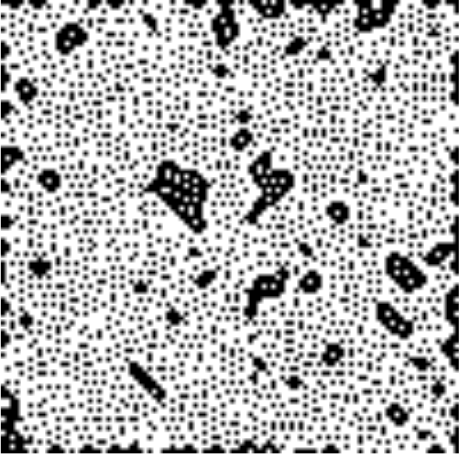
\includegraphics[width=.2\textwidth]{images/pclass1.png}}\hfill
            \subfloat[B12345678/S234]{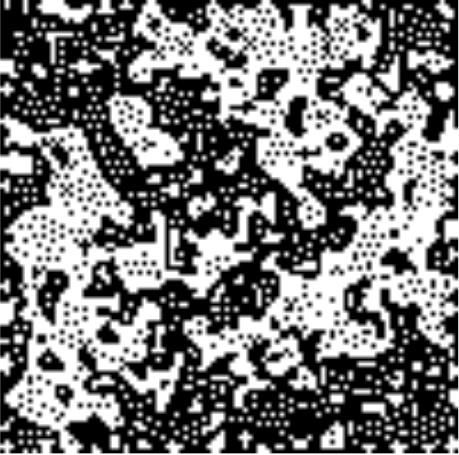
\includegraphics[width=.2\textwidth]{images/pclass2.png}}\hfill
            \subfloat[B1/S345]{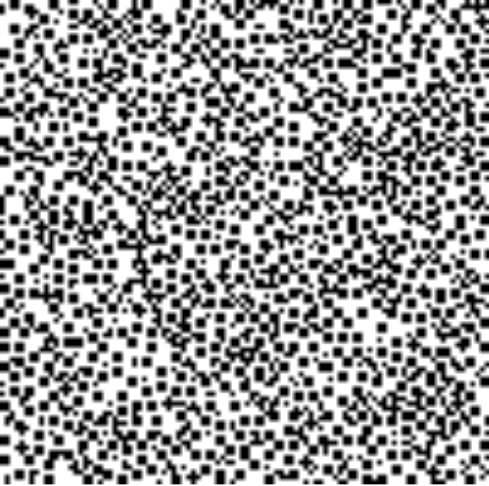
\includegraphics[width=.2\textwidth]{images/oclass1.png}}\hfill
            \subfloat[B1/S345678]{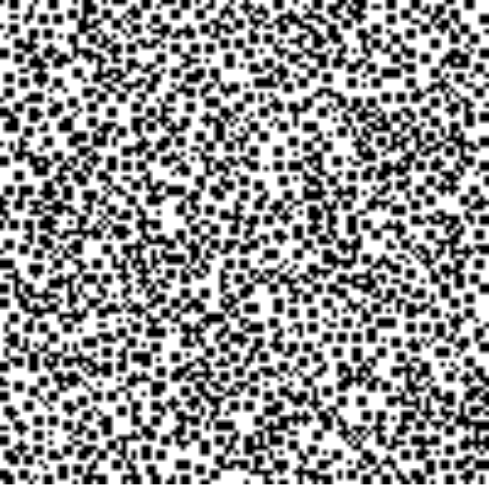
\includegraphics[width=.2\textwidth]{images/oclass2.png}}
            \caption{Configurations generated from P-class (a,b) and O-class (c,d) rules \cite{adamatzky2006phenomenology}}
\label{fig:po-class}
\end{figure}

Adamatzky et al.\cite{adamatzky2006phenomenology} produces a systematic analysis of a subset of life-like CA where birth and survival sets are contiguous intervals. These are dubbed "binary-state reaction-diffusion cellular automata (RDCA)" as they provide a discretized simulation of simple substrate-reagent reactions. The analysis includes categorisations based on qualitative factors like the features and density of resulting configurations and quantitative factors like the outcome of glider collisions within each universe. For example, the \textbf{P}-class contains rules with high diffusion rate (i.e. wide birth interval) and low reaction rates (i.e. narrow survival interval) which produce large regions of 0-state and 1-state each containing scatterings of the other within them. These patterns are qualitatively distinct from, for example, \textbf{O}-class rules which have low diffusion rate and high reaction rate producing irregular spotted patterns. Despite the depth of this investigation, the 1296 CA rules analysed cover less that 0.05\% of all life-like CA. A broader issues in both Wolfram's and Adamatzky's classifications is the lack of objective distinction between class boundaries which makes it difficult to predict the behaviour of rules \textit{a priori}. Indeed, some automata have been proven to span multiple classes\cite{baldwin1999classi}.\\

This dilemma is alleviated to some degree by Eppstein's four-way classification\cite{eppstein2010growth} which is based on strict definitions of \textit{fertility} and \textit{mortality}. A rule is fertile if there exists a finite pattern that eventually escapes any bounding box B. Note this is symmetrically opposite to the definition of periodicity since any infertile rule can only iterate through $2^{|B|}$ steps before repeating a previous state. A rule is mortal if it supports a pattern which transitions to the \textit{quiescent} state (i.e no live cells) in the next time step. Eppstein conjectures that "interesting" behaviour arises out of rules that are both fertile and mortal. Figure~\ref{fig:eppstein-map} depicts a schematic map of his analysis.\\

This work provides a strong theoretical foundation to guide our search of life-like CA and to verify that our techniques are effective on different varieties. However, they are not grounded in a systematic statistical search to reveal the proportion of each category that exist in contested regions. For example, we may be interested in the ratio of fertile to infertile configurations for B3/S01. Although a closed-form solution for this ratio is infeasible, it is possible to come to an approximation through simulation. Soup searches are large scale simulations of random initial conditions on particular rules typically used to identify new patterns. In a similar vein, we will use soup searches to approximate the fertility and periodicity of all rules in the life-like CA rulespace.

\begin{figure}[!h]
\centering
    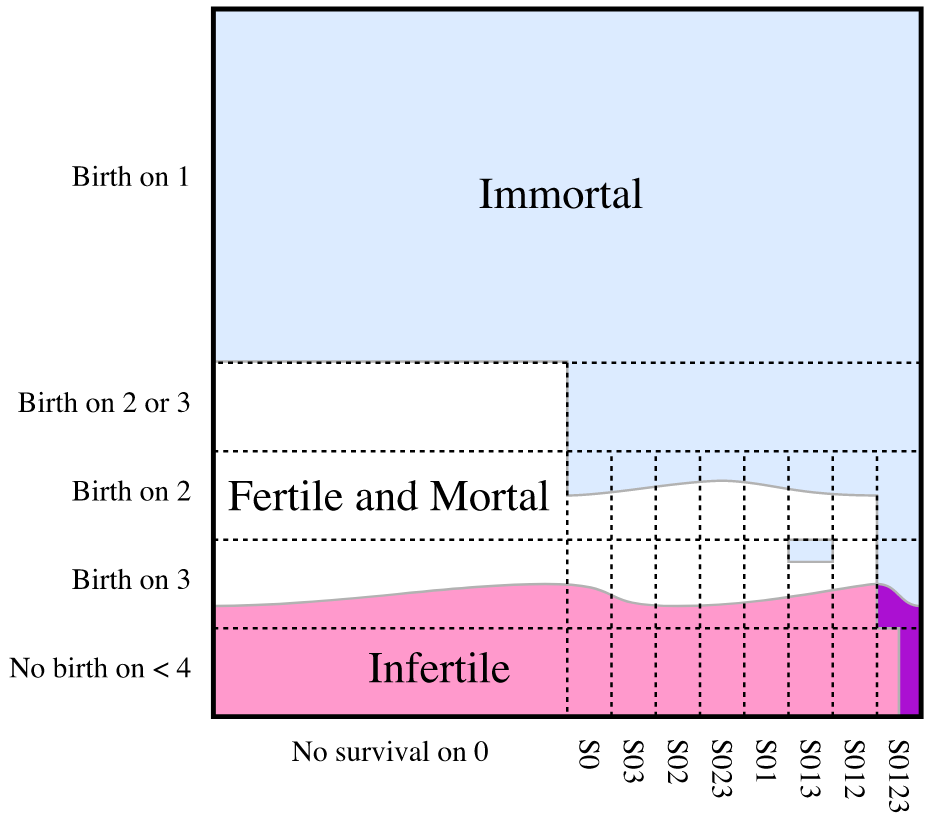
\includegraphics[width=.5\textwidth]{images/eppstein-map.png}
    \caption{Map of fertile, infertile, mortal, and immortal regions in binary-state RDCA rulespace \cite{eppstein2010growth}}
\label{fig:eppstein-map}
\end{figure}

\subsection{Learning}

\noindent
\textbf{Learning Algorithm for Modeling Complex Spatial Dynamics} (Meyer et al., 1989) \cite{meyer1989learning} is a seminal work that uses genetic algorithms to learn cellular automata neighbourhood functions. It evolves a binary probabilistic cellular automaton (PCA) to model artificially generated datasets. The motivation is to establish a CA architecture to codify patterns in physical interactions directly from experimental data. In particular, Richards et al. \cite{richards1990extracting} uses PCA rules to predict the the dendritic solidification structure of NH\textsubscript{4}BR.\\

Note that the goal is not to learn the entire transition function of the cellular automaton. This work aims to establish \textit{which} parameters in a local vicinity of a current cell are most relevant to predicting the future state, not \textit{how} those parameters are combined and transformed to produce the result.\\

The search space is a 20-cell vicinity where each cell can be included or excluded from the neighbourhood set. It is the intersection of the Moore neighbourhood in time step $t-1$ and the von Neumann neighbourhood of range 2 in time step $t-2$ as visualised in Figure~\ref{fig:20-near}.

\begin{figure}[!h]
\centering
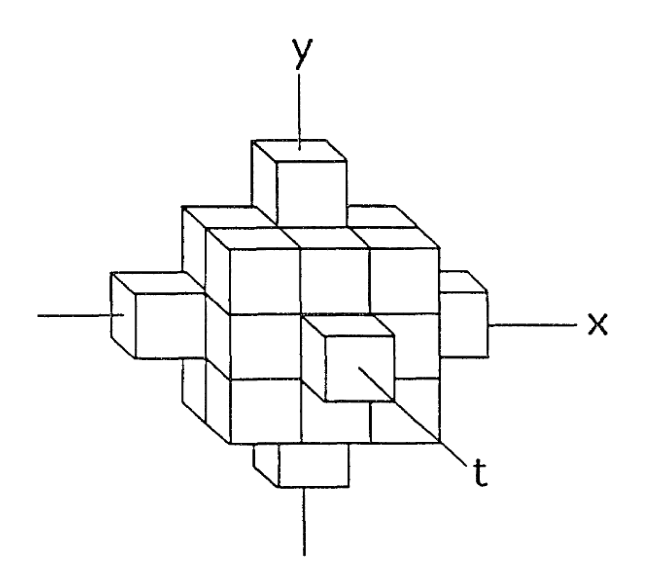
\includegraphics[width=0.3\textwidth]{images/20_neighbourhood.png}
\caption{20-cell, two step neighbourhood in space and time}
\label{fig:20-near}
\end{figure}

The full 20-cell neighbourhood is called the master template and each chromosome encodes some subtemplate ${s_1, ..., s_m}$. The fitness function used is
\begin{align*}
                    F &= I - \frac{2^m}{N}\\
    \text{where\:}  I &= \sum P(s, s_1, ..., s_m)\log_2{\frac{P(s, s_1, ..., s_m)}{P(s)P(s_1, ..., s_m)}}
\end{align*}
Here, $I$ is the mutual information of the subtemplate and represents the amount of information, measured in Shannon bits, that can be obtained about the value of the central cell from subtemplate states. It is calculated by summing across all $2^m$ configurations of the subtemplate in the data and across both values of $s \in \{0,1\}$. The second term in the fitness function ensures that subtemplates of varying sizes are treated appropriately by proportionately penalising large subtemplates that, by nature, will contain more information. $N=20$ is the size of the master template\\

The genetic algorithm initialises the population at a randomly chosen subset of possible subtemplates. Selection is performed using a truncated linear ranking. Crossover is applied using an arbitrary cut in space-time on the master template as the crossover point. Point mutation is applied by either adding or removing a single cell from each candidate. This process is iterated to converge towards an optimum.\\

This method precisely learns neighbourhoods interior to the master template such as the 1 time step Moore neighbourhood. Even when the objective neighbourhood lies partially outside the master template, the algorithm successfully finds a close approximation. For example, when given data produced by a 1 time step von Neumann neighbourhood, the algorithm learns a neighbourhood set that produces correct behaviour 96\% of the time.\\

As the first notable exploration of learning CA properties with genetic algorithms, this paper demonstrates the ability of GAs to efficiently traverse an opaque search space and approximate solutions to goals outside the search space.\\

This work also raises many questions for future research. The most pertinent is whether it is possible to link learned rules to existing and future theoretical models. Moreover, this work only explores binary state CA but application of similar techniques on continous-state CA could closer approximate the partial differential equations that underlie the physical processes being modelled.\\

Finally, this paper focuses on optimising the neighbourhood set of the CA model only. In this thesis, we are interested in going beyond this and approximating the full transition function. In some cases we will fix the neighbourhood function used to reduce our search space under the assumption that techniques from this paper can be used to find optimal sub-neighbourhoods if they exist.\\

\noindent
\textbf{Evolving Cellular Automata with Genetic Algorithms} (Mitchell, Crutchfield, and Das, 1996) \cite{mitchell1996evolving} shows the effectiveness of genetic algorithms in learning elementary cellular automata for global learning tasks such as the infamous density classification[CITE] and synchronisation[CITE] problems.\\


\section{Continuous Reaction-Diffusion CA}